\section{John Backus and Fortran}

IBM did not feel that Aiken and the Harvard Computation Laboratory had given
them sufficient credit for their contributions to the Mark I, which left
Thomas Watson Sr. and the IBM folks bitter about the experience and eager to
produce a new device entirely in-house. This device would become the Selective
Sequence Electronic Calculator, or the SSEC. It was built on 57th Street in
Manhattan, and it was monstrous. Roughly 50 by 100 feet with a giant console
and hundreds of toggle switches and tape units and relays behind glass panels;
there were giant windows that allowed passersby to see the machine in action.

One such passerby was John Backus, a recent Masters graduate from Columbia
University. He was intrigued by the machine, which he mentioned to his tour
guide, who suggested he go upstairs and talk to the boss about it. Robert "Rex"
Seeber gave him a puzzle, which he solved, and he was hired on the spot
\cite{backus_oral_history_2006}.

In 1942, Backus majored in Chemistry at the University of Virginia where he
struggled academically. He was expelled due to poor attendance within the first
year before being drafted into the US Army. He commanded an antiaircraft
battery at Fort Steward, Georgia, remaining in the US for the remainder of
WWII.

While he did not at first find success in academia, he got very good marks on
military aptitude tests. He was directed to the University of Pittsburgh's
engineering program and later to a premedical program at Haverford College near
Philadelphia (which is where he grew up). In 1945 he attended the Flower and
Fifth Avenue Medical School in NYC, but he was still struggling with the
academy. He was uninterested in medicine, feeling that it was all about
memorization. He dropped out after less than a year.

He entered a radio technician school and became interested in math, which led
him to enroll in the math program at Columbia University. The SSEC that would
intrigue him at the IBM computing center was designed at the Watson Scientific
Computing Laboratory at Columbia.

\subsection{Speedcoding to FORTRAN}

At IBM, Backus worked on the SSEC and later the IBM 701 and 704. The main use
of the SSEC was aerospace calculations; programming calculations to predict the
position of the moon was one of the first tasks he was given at IBM. He would
continue writing programs for these machines in spite of their poor usability.
His team's techniques would be used in the lunar missions of the 1960s.

The pain of writing programs for these early machines entirely in machine code
drove him to explore new ways to program. The first of these was a symbolic
notation for floating point arithmetic and address expression calculation
called Speedcoding\cite{backus_oral_history_2006}:

\begin{quotation}
	\textbf{Grady Booch:}
	So then from your experience with the SSEC, you then went on to
	produce Speedcoding, the
	Speedcoder\dots
	What were sort of the things that influenced you to create that in
	the first place?

	\textbf{John Backus:}
	Well, programming in machine code was a pretty lousy business to
	engage in, trying to figure
	out how to do stuff. I mean, all that was available was a sort of a
	very crude assembly program. So I
	figured, well, let's make it a little easier. I mean it was a
	rotten design, if I may say so, but it was better
	than coding in machine language.
\end{quotation}

The IBM 701 did not have an index register, so calculating addresses for array
operations was tedious and error-prone. Speedcoding provided a way to express
these calculations symbolically.

\begin{figure}[h!]
	\centering
	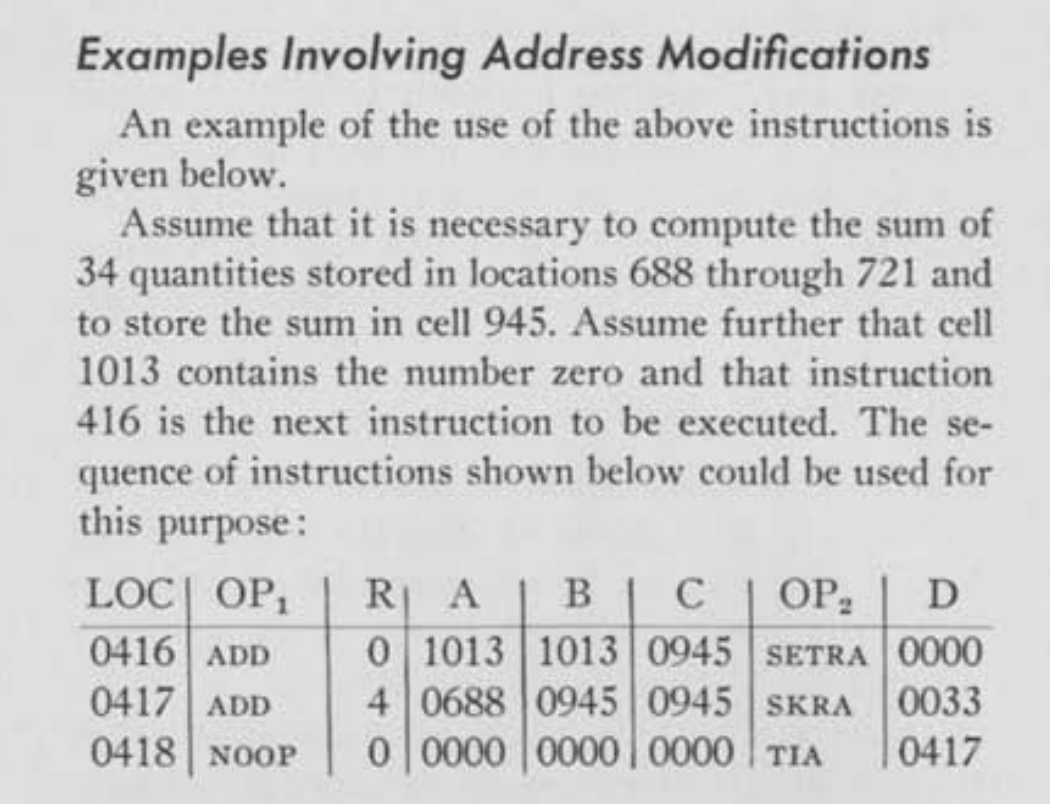
\includegraphics[width=0.5\linewidth]{resource/ibm-speedcoding-example.png}
	\caption{Excerpt from \textit{IBM Speedcoding for the Type 701
			Electronic Data Processing Machine}
		\cite{IBM_1954_Speedcoding}}
	\label{fig:ibm-speedcoding-example}
\end{figure}

The 704 was the first machine to have such a register; it also had floating
point instructions and core memory, more or less obviating the need for
Speedcoding: "we were moving to the 704, which had built in floating point,
built in index registers, which was all that Speedcoding was supposed to
supply. So what the hell?" \cite{backus_oral_history_2006} He credits himself
with getting index registers and floating point into the 704.

%Here is an example from the IBM Speedcode manual\cite{IBM_1954_Speedcoding}:
%\begin{quotation}
%    Assume that it is necessary to compute the sum of 34 quantities stored in
%    locations 688 through 721 and to store the sum in cell 945.
% Assume further that
%    cell 1013 contains the number zero and that instruction 416 is the next
%    instruction to be executed. The sequence of instructions shown
% below could be
%    used for this purpose:
%
%    \begin{center}
%    \begin{tabular}{cccccccc}
%    \hline
%    LOC & OP$_1$ & R & A & B & C & OP$_2$ & D \\
%    \hline
%    0416 & ADD  & 0 & 1013 & 1013 & 0945 & SETRA & 0000 \\
%    0417 & ADD  & 4 & 0688 & 0945 & 0945 & SKRA  & 0033 \\
%    0418 & NOOP & 0 & 0000 & 0000 & 0000 & TIA   & 0417 \\
%    \hline
%    \end{tabular}
%    \end{center}
%\end{quotation}

Backus did not think all that highly of Speedcoding in retrospect, though it
gained traction in large part due to IBM's marketing power and the number of
users of the 701 relative to the size of the computer market at the time
\cite{Backus_1980_Programming_in_America_in_1950s}. It is unclear whether
Backus's assessment of his own code is accurate or if it's born of humility.

\begin{quotation}
	The success of some programming systems depended on the number of machines
	they would run on. Thus, an elegant system for a one-of-a-kind machine might
	remain obscure while a less-than-elegant one for a production
	computer achieved popularity.

	This point is illustrated by two papers at the 1954 ONR symposium
	One, by David E. Muller, describes a floating point interpretive system for
	the ILLIAC designed by D. J. Wheeler. The other, by Harlan Herrick and myself,
	describes a similar kind of system for the IBM 701 called Speedcoding. Even
	today Wheeler's 1954 design looks spare, elegant, and powerful, whereas the
	design of Speedcoding now appears to be a curious jumble of compromises.
	Nevertheless, Wheeler's elegant system remained relatively obscure (since only
	ILLIAC users could use it) while Speedcoding provided enough conveniences,
	however clumsily, to achieve rather widespread use in many of the eighteen 701
	installations.
\end{quotation}

In 1953, based on his experience with Speedcoding on the 701, Backus proposed
yet another language to elevate the programming experience on the 704. IBM
management supported the proposal. He formed a ten-person team of his own
choosing based out of IBM's Manhattan headquarters, including Irving Ziller,
\todo{list other members}. They released \citetitlecite{IBM_1954_FORTRAN_Specifications}
after about one year of working
together.
Roughly two years after its first conception, \FTN{} was released for
the first time. It would go on to ship with every IBM 704 and become the
primary means of programming in the scientific community.

Backus could not
stand how slow programming was without a higher-level language, and machines
were expensive; leasing a machine and spending time programming in machine code
wasted money compared to a compiler capable of generating reasonable machine
code (though at the time it usually underperformed hand-written code). Backus
and his team would continue to develop and stabilize this compiler for several
years, though.

\begin{quotation}
	\FTN{} did not really grow out of some brainstorm about the beauty of
	programming in mathematical notation; instead it began with the recognition
	of a basic problem of economics: programming and debugging costs already
	exceeded the cost of running a program, and as computers became faster
	and cheaper this imbalance would become more and more intolerable. This
	prosaic economic insight, plus experience with the drudgery of coding, plus
	an unusually lazy nature led to my continuing interest in making
	programming easier.
	This interest led directly to work on Speedcoding for the 701
	and to efforts to have floating point as well as indexing built into the 704.
	\cite{Backus_1980_Programming_in_America_in_1950s}
\end{quotation}

When Backus was forming his team in January of 1954, he was moved from the Pure
Science department at IBM into the Applied Science department because his boss
Rex Seeber wanted nothing to do with the project. There he found Irving Ziller,
who became his first teammate. By April, they had been joined by Harlan Herrick
who co-authored the Speedcoding paper with Backus at the ONR symposium
\citetitle{Backus_Herrick_1954_Speedcoding} in which they observe:

\begin{quotation}
	The question is, can a machine translate a sufficiently rich mathematical
	language into a sufficiently economical program at a sufficiently low cost to
	make the whole affair feasible?  consider the advantages of being
	able to state
	the calculations\dots for a problem solution in a concise, fairly natural
	mathematical language.
\end{quotation}

The reader should note that it is often incorrectly asserted (at times even by
Backus himself\cite{Backus_1980_Programming_in_America_in_1950s}) that this
came \textit{after} Backus and Ziller had been given a demonstration of Laning
and Zierler's algebraic compiler for the Whirlwind at MIT at the ONR symposium
of 1954. When they received this demonstration, there were already four members
of the \FTN{} team, Irving Ziller, Robert Nelson, Harlan Herrick, and Backus
himself. In Backus's words\cite{Backus_1980_Programming_in_America_in_1950s}:

\begin{quotation}
	The article and the letter therefore show that, much to my surprise, the
	FORTRAN effort was well under way before the ONR symposium and that,
	independently of Laning (but later), we had already formulated more ambitious
	plans for algebraic notation (e.g., Gail bjk) than we were later to find in
	Laning and Zierler's report and see demonstrated at MIT. It is therefore
	unclear what we learned from seeing their pioneering work, despite my mistaken
	assumption over the years that we had gotten our basic ideas from them
\end{quotation}

Indeed, even Grace Hopper made the same assertion at a 1956 symposium:

\begin{quotation}
	A description of Laming and Zierler' s system of algebraic pseudocoding for
	the Whirlwind computer led to the development of Boeing 's BACAIC for the 701,
	FORTRAN for the 704, AT-3 for the Univac, and the Purdue System for the Datotron and
	indicated the need for far more effort in the area of algebraic
	translators.
	\cite{Knuth_TrabbPardo_1976_Early_Development}
\end{quotation}

Donald Knuth and Trabb Pardo quote her in \citetitle{Knuth_TrabbPardo_1976_Early_Development}
as well.
I am not sure who to believe either!

With the support of his new boss Cuthbert Hurd, his family, friends, and his
team, the first report of \FTN{} was released externally to 704 users. This
brought interest from a variety of users, many of whom offered up members of
their teams to help.

The original FORTRAN report had some peculiarities and made some large claims,
some of which came true and some of which \textit{very much} did not.
Variables had one or two characters, function names of three or more characters,
and array variables with up to three subscripts.
The document used the term \textit{arithmetic formulas} to describe what
we would today call \textit{assignment statements}.

\begin{figure}[h!]
	\centering
	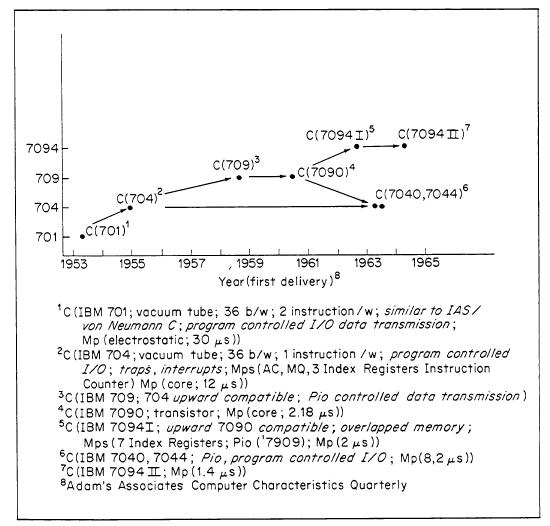
\includegraphics[width=0.5\linewidth]{resource/ibm-7094.jpeg}
	\caption{Excerpt from \textit{The IBM 701--7094 II Sequence: A
			Family by Evolution}
		\cite{Hamming_Feigenbaum_1971_IBM7094}, illustrating the
		instruction structure for summing quantities.}
	\label{fig:ibm7094-example}
\end{figure}

DO formulas were particularly interesting, and not necessarily the construct that we
today call \textit{loops}.
Any \textit{formula} could have an associated number with it, allowing that formula to be
invoked from elsewhere in the program.
For example, in the following snippet taken from the original report,
the formulas starting with 10 and ending with 14 would be executed
9 times in total, starting with i taking the value of 4 and incrementing by 2
until reaching 20; once completed, control resumes at formula 30:

\begin{lstlisting}[language=fortran,frame=single]
      do 10 14 30 i=4,20,2
\end{lstlisting}

Whew! For such a fundamental concept, the \gls{cfg} is potentially very complex.
I suspect that in most cases, only one or two formulas were specified.
When the third formula number is omitted, execution resumes at the instruction
immediately following the final formula of the DO construct, and
if only one formula is specified, then that is the last formula to execute,
and the first is the one immediately following the DO statement.

Another peculiar feature was the RELABEL formula, which was intended to make
matrix rotation operations simpler. For example, for a 4x4 matrix \texttt{b}, the
formula \texttt{RELABEL(3,1)} would result in \texttt{b(1,i)} taking the same meaning as \texttt{b(i,1)}
had prior to the relabel.
There soon came better ways to express the same idea, and I am unable to find any example
programs using this construct, even in the original report.

The final section of the report notes that "no special provisions have been included
in the FORTRAN system for locating errors in formulas\dots
Since FORTRAN formulas are fairly readable, it should be possible to
check their correctness by independently recreating the specifications for
the problem from its FORTRAN formulation." \cite[C. DEBUGGING]{IBM_1954_FORTRAN_Specifications}
It is remarkable that they \textit{did} consider how to debug FORTRAN programs,
and then \textit{thought better} of providing error messages.

Again, they were tragically optimistic: in the second page of the report,
they claimed that "FORTRAN should virtually eliminate coding and debugging."

\subsection{The Priesthood}
\label{sec:backus_priesthood}

At this time, it was not obvious to everyone in the industry that
programming languages were needed at all--a large consortium of programmers
thought that machine code was all anyone would ever need.
Backus would later describe this group in \citetitle{Backus_1980_Programming_in_America_in_1950s}:

\begin{quotation}
	Just as freewheeling westerners developed a chauvinistic pride in their frontiersmanship
	and a corresponding conservatism, so many programmers of the freewheeling 1950s
	began to regard themselves as members of a priesthood guarding skills and
	mysteries far too complex for ordinary mortals.
	\cite{Backus_1980_Programming_in_America_in_1950s}
\end{quotation}

In the Office of Naval Research's 1954 symposium,
\citeauthor{brown_carr_automatic_onr_symposium_1954} summarize the recent developments
of \textit{automatic programming} techniques like \textit{pre-translation} and \textit{running-translation},
or compilers and interpreters.
Their depiction also described the opposition to the development of more friendly
input formats for computers, not yet even discussing programming languages:

\begin{quotation}
	Many "professional" machine users strongly opposed the use of decimal
	numbers for computer inputs or outputs as being unnecessary. Often they felt
	that direct binary (or associated octal or hexadecimal) coding of instructions
	was the only possible method. To this group, the process of machine instruction
	was one that could not be turned over to the uninitiated.
	\cite{brown_carr_automatic_onr_symposium_1954}
\end{quotation}

At each step in the development of compilers and programming languages,
a non-negligible subset of the programming community has resisted the move
towards user-friendliness, and the sentiment \citeauthor{brown_carr_automatic_onr_symposium_1954}
described above is perhaps the first.
\footnote{
	Perhaps engineers working on the ENIAC resisted accessibility as well:
	"real engineers plug the phone lines of the computer! Punch-card programs are for sissies!"
}

Backus recalled that this sentiment disuaded efforts towards accessibility:
"[t]he priesthood wanted and got simple mechanical aids for the clerical
drudgery which burdened them, but they regarded with hostility and derision
more ambitious plans to make programming accessible to a larger population."
He and Bill Heising would later recall (emphasis added):

\begin{quotation}
	At that time, most programmers wrote symbolic machine instructions exclusively
	(some even used absolute octal or decimal machine instructions).
	Almost to a man, they firmly believed that any mechanical coding method
	would fail to apply that versatile ingenuity which each programmer felt he
	possessed and constantly needed in his work.
	Therefore, it was agreed, \textbf{compilers could only turn out code which would be
		intolerably less efficient than human coding}\dots
\end{quotation}

Setting aside the emotional arguments against programming languages and making
computing more accessible, Backus had very practical and economic reasons as well.
He noted that the most costly part of computing was becoming the development of
software. In the early days of computing, the cost of the hardware was so
astronomically high and the standard for software was so low that the development of software
was an afterthought--the organization leasing the computer could easily find
programmers to write whatever programs they cared about, and the cost would be
a tiny fraction of the cost of the hardware.

As the machines themselves became cheaper and more powerful and the scale of software
increased, the cost of software development became more and more important.
This will be the focus of Chapter \ref{chap:software}.
The key players on the side of the debate that favored accessibility and
programming languages were John Backus, Grace Hopper, J. Halcombe Laning,
and Neil Zierler, along with their respective teams.

The sentiment of the priesthood may seem antiquated, but it seems to be
present in one form or another in every chapter of this history of programming languages
and compilers, and it had a notably positive influence on the development of FORTRAN:
because FORTRAN would face significant resistance if it could not produce
efficient machine code, Backus, Ziller, and their team devoted a huge amount of
effort towards optimization.
Their primary fear was that after spending much effort building a FORTRAN
compiler, an important application would be written in FORTRAN and turn
out to run at half the speed of the machine-coded version, and the
sceptics would be right\cite{backus_heising_fortran_1964}.

Their work would be foundational for modern optimization techniques, and
FORTRAN compilers continue to produce extremely efficient machine code to
this day, in part because the language's design allows for a high degree of
optimization, and in part because compiler engineers have been optimizing
FORTRAN programs for longer than any other programming language.

\subsection{FORTRAN I}

In 1956, they released the reference manual \citetitlecite{backus_fortran_ref_manual_1956} with a FORTRAN
that looked very similar to the original, with a few deletions and minor changes.
The ill-fated \texttt{RELABEL} formula was removed and the \texttt{DO} statement was simplified.
Instead of taking potentially three formulas (the first, last, and continuation formulas),
one now only specified the final formula of the loop, or the \gls{backedge}.

In the following loop, \texttt{I} begins at 1 and increments by 1 until it reaches 5, and for
each iteration, \texttt{N(I)} is accessed, multiplied with \texttt{I} and stored in \texttt{A(I)}:

\begin{lstlisting}[language=Fortran,frame=single]
10    DO 20 I=1,5
20    A(I) = I*N(I)
30
\end{lstlisting}

IF-statements were still quite unweildy; they took three formulas, the first if the
condition yielded a negative value, the second if it was zero, and the third if it was positive:

\begin{lstlisting}[language=Fortran,frame=single]
10    IF(A(I)) 20,30,40
20    ! ... Jump to here if A(I) < 0
30    ! ... Jump to here if A(I) = 0
40    ! ... Jump to here if A(I) > 0
\end{lstlisting}

To be fair to John Backus, he is quite self-deprecating when recalling these details about the
language design process.

\begin{quotation}
	Since our entire attitude about language design had always been a
	very casual one, the changes we felt to be desirable during the course
	of writing the compiler were made equally casually\dots

	In our naive unawareness of language design problems--of course,
	we knew nothing of many issues that were later thought to be important,
	e.g., block structure, conditional expressions, and type declarations.
\end{quotation}

At this time, Backus, Herrick, Ziller, and their team at IBM were shopping around
their compiler and programming language to potential customers of the IBM 704.
Their primary purpose was to collect aspects of the system that their customers found
confusing or objectionable, or aspects they felt were missing.
In late 1954 and early 1955, they gave talks to these customers and recieved next to
no helpful feedback.
It seemed that too frequently, customers had been systems with lots of promise, only to
finally recieve an unweildy or peculiar system with restrictions that were not mentioned
during the sales process.

The first significant payoff from these talks came in January 1955 when they visited the
United Aircraft Corporation. Roy Nutt was leased out by his boss Walter Ramshaw
to IBM to work on the input/output
libraries for FORTRAN, and he would visit New York several times a week to collaborate with
the team until 1957.
Charles Adams from MIT allowed Sheldon Best to join the team,
and Sidney Fernback from Livermore Radiation Laboratory joined as well.

Backus remarks that while his team could have been better salespeople and that
Laning and Zierler's compiler was more influential and compelling at the time, the early FORTRAN efforts
likely influenced at least the development of Hopper's Math-Matic compiler at
Sperry Rand.
If they did not convince users of the utility of their new compiler and programming language,
they at least picked up new contributors that would go on to make large contributions.

\subsection{Their First Compiler}

In early 1955 when development on their compiler began, it was only referred to as their \textit{translator}.
Herrick wrote lots of test programs to feel out the language, and the team had an ad-hoc understanding of the
sort of code they expected to get from various source programs, though their language lacked a
rigorous specification.
The team broke into smaller teams of one to three people, each responsible for a section of the compiler.
Each group agreed on the input and output formats to be used on the boundaries of their component and what came before and after.

\begin{figure}[h]
	\centering
	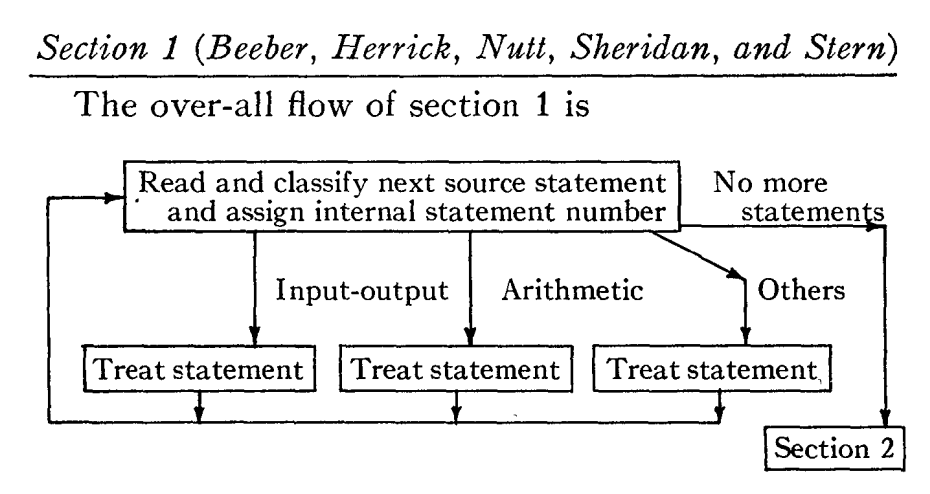
\includegraphics[width=0.8\textwidth]{resource/dawn/backus-fortran-sec-1.png}
	\caption{Section 1 of the Original FORTRAN compiler\cite{backus_etal_fortran_automatic_coding_system_1957}}
	\label{fig:backus_fortran_compiler}
\end{figure}

Their \textit{translator} was a single-pass compiler.
The first section (see Figure \ref{fig:backus_fortran_compiler}) of the compiler
consumed the entire program, produced machine code for what it could,
and left the rest of the information about the source program in lookup tables
for the other sections of the compiler.
We would likely call this the front-end of the compiler as it composed
parsing and a bit of semantic analysis.

In section 2, some parts of the user's program (particularly I/O statements)
would be transformed into DO-statements, which would then still need to be compiled.
This section also performed some optimization steps, including \gls{licm} and
register allocation.
The optimizations in section 2 were primarily invented by Robert Nelson and Irving Ziller.
These optimizations originally included register allocation \textit{for the entire program},
until Backus proposed that the earlier phases of the compiler should assume the
target machine (at this point only the IBM 704) has unlimited index registers,
and later phases of the compiler would finish the job of register allocation.

This proposal neccesitated sections 4 and 5, and section 3 to translate the
output of the first two sections into the format section 4 expected.
Lois Mitchell Haibt joined the group to design and program section 4,
which was responsible for some significant analyses.
Section 2 would be responsible for constructing and analyzing the \gls{cfg}
of the user's program, breaking the program into \gls{basicblock}s,
and \textit{performing a Monte-Carlo simulation} of the user's program
based on DO-statements and optimization hints in the form of FREQUENCY statements
to track how often each basic block was used, and to collect utilization
statistics on the program's index registers.

Wow! That must have been a massive undertaking.
Aside from inventing new compiler optimization techniques, this is the first
instance I can find of \gls{pgo}.
They quickly ran into tradeoffs between compile-time spent in analyses and optimizations
and the actual differences in performance these analyses brought to the user's
program.
In once instance, a sub-component of the register allocation analysis took ten minutes
of the twenty total minutes in compile time,
even though the program used no index registers--thus half the compile time
went towards analyses that made no difference in the final program
\cite{backus_heising_fortran_1964}.

Section 5 was then responsible for leveraging the analyses from section 4
to perform register allocation for the 704's three index registers.
This section was designed and implemented by Sheldon Best from MIT,
who was on loan as a temporary IBM employee.
Best's methods would become the basis for register allocation research for many years to come.

It was not obvious to the team until later in 1955 that a section in
between 2 and 4 would be needed; Richard Goldberg joined in November of 1955,
and he designed and implemented this section,
and took over section 5 from Best after he returned to MIT.

Section 6 was naturally designed by Nutt, as he wrote the I/O runtime libraries
for the original compiler, and section 6 assembled, linked, and loaded the final program.
For such an I/O-heavy portion of the compiler, he was the natural choice.
Thanks to the efficient I/O features Nutt added to the language, this section
was many times faster than competing assemblers and linkers.

From mid 1956 to early 1957, the focus was on bringing the compiler to market.
They would rent out a hotel near the headquarters to sleep during the day
so they could debug their new compiler all night long while it sat unused by other
teams.
The team started surprising themselves with the transformations their compiler
was capable of; the optimization gurus Nelson and Ziller would always be able to figure
out how the compiler determined the transformation was correct and beneficial, but
it was still a surprise to see all the pieces come together.

In 1957 they published a small addendum to the Programmer's Reference Manual,
documenting \textit{functions statements}, which have persisted through to modern Fortran.
They allow users to define functions in a single statement, like so:

\begin{lstlisting}
FIRSTF(X) = A*X+B
SECONDF(X, B) = A*X+B
THIRDF(D) = FIRSTF(E)/ D
FOURTHF(F,G) = SECONDF(F, THIRDF(G))
\end{lstlisting}

There were numerous language features specific to the 704 as well,
such as the SENSE LIGHT statement, which toggled specific sensor lights:

\begin{quotation}
	\begin{tabular}{|c|c|}
		\hline
		GENERAL FORM                                 & EXAMPLES      \\
		\hline
		"SENSE LIGHT i" where i is 0, 1, 2, 3, or 4. & SENSE LIGHT 3 \\
		\hline
	\end{tabular}
\end{quotation}

The PUNCH statement was also present in the handbook, which allowed users to
directly use the card-punching attachment on the 704.

Among the optimization efforts, Nelson and Ziller optimized array indexing expressions and
wrote loop analysis passes.
Backus specifies that they could "could move computations from the object
program to the compiler" which appears to be the first instance of
\gls{constant-folding} in a compiler.

In the spring of 1957, they published \citetitle{backus_etal_fortran_automatic_coding_system_1957}
and they distributed it to every IBM 704 customer.
After lots of debugging in the field and difficulties punching out copies
of the compiler, it was not long before most of the installations were using it.
By fall of 1958, more than half of the machine code produced at the roughly 70 installations
with an IBM 703 or 704 were being produced by their FORTRAN compiler.

\subsection{Optimizing FORTRAN I}

Driven by the fear of the sceptics' fears coming true and delivering a FORTRAN compiler
that produced programs significantly slower than their hand-coded equivalents,
they tried to evaluate which parts of a program would be most subject to inefficiencies.
One of the first considerations was the calculation of \textit{addressing expressions}
\cite{backus_heising_fortran_1964}
(which continues to be a challenging optimization problem).
This will be explained further below.

When a program iterates over the elements of a matrix $A_{m, n}$ with $m$ rows and $n$ columns in a loop,
the element of $A_{i, j}$ is accessed in column-major order with the following calculation:

\[
	A_{i, j} = \text{base-address}(A) + ((i - lbound(A, 1)) + m \times (j - lbound(A, 2))) \times s
\]

where $s$ is the number of bytes in an element of $A$, and $lbound$ gives the lower bound of the array
for a given dimension.
In many cases, the lower bound of all dimensions is $1$, which gives a more straightforward calculation:

\[
	A_{i, j} = \text{base-address}(A) + ((i - 1) + n \times (j - 1)) \times s
\]

And even more simply, the offset of an index from the base address of a matrix
with all-one lower bounds measured in units of the size of an element is simply:

\[
	A_{i, j} = (i - 1) + n \times (j - 1)
\]

If the loop accesses the elements of $A$ such that each element resides immediately next to the previous
element in the innermost loop, then the compiler can re-use the address calculation from the previous
iteration of the innermost loop.

More concretely, here we see the elements of our matrix $A$:
\[
	A =
	\begin{bmatrix}
		a_{1,1} & a_{1,2} & \cdots & a_{1,N} \\
		a_{2,1} & a_{2,2} & \cdots & a_{2,N} \\
		\vdots  & \vdots  & \ddots & \vdots  \\
		a_{M,1} & a_{M,2} & \cdots & a_{M,N}
	\end{bmatrix}
\]

Thus the elements are laid out in memory as a contiguous block of memory:

\[
	\big(
	a_{1,1},\; a_{2,1},\; \dots,\; a_{M,1},\;
	a_{1,2},\; a_{2,2},\; \dots,\; a_{M,2},\;
	\ldots,\;
	a_{1,N},\; \dots,\; a_{M,N}
	\big)
\]

So, a FORTRAN program accessing elements of $A$ linearly as they
are stored in memory (also known as \gls{stride1})
\href{https://godbolt.org/z/T6M4dvMP4}{would look like this:}

\begin{lstlisting}[language=Fortran,frame=single]
      real A(3,3)
      integer i,j
c     Innermost loop is the fastest-moving index
      do 10 j = 1, 3
         do 10 i = 1, 3
            A(i,j) = real(i)/real(j)
            print *, i, j
   10 continue
      end

c     Program prints:
c     1           1
c     2           1
c     3           1
c     1           2
c     2           2
c     3           2
c     1           3
c     2           3
c     3           3
\end{lstlisting}

Now, the FORTRAN team's concern was that their compiler would not be able to recognize
that a program like the one above was accessing memory in a way consistent with the
way arrays are stored in memory, and would miss the fact that in calculating
the address of an array element $A_{i,j}$ for $i > 1$, parts of the address calculation
for index $A_{i-1, j}$ could be re-used and $A_{i-1, j}$ and $A_{i, j}$ reside
next to each other in memory.

Because programmers writing machine code would naturally do this and FORTRAN
programs would spend much of their time in loops iterating over matrices,
it was critical that their compiler be able to recognize this idiom.
After scoping out the problem, they found the space of possible address calculation
expressions to be very large indeed.

For example, in the loops above, it is obvious that the matrix $A$ is accessed
with \gls{stride1} because the innermost loop iterates over the columns of the
matrix, and the \gls{inducvar} $i$ is incremented by one via the DO loop,
and is not modified in the loop body.
Consider the following program, where it is not \textit{quite} so clear:

\begin{lstlisting}[language=fortran,frame=single]
      real A(3,3)
      integer i,j
c     Innermost loop is the fastest-moving index
      do 10 j = 0, 2
         do 10 i = 1, 3
            i = i + 1
            A(i,j) = real(i)/real(j)
            print *, i, j
   10 continue
      end
\end{lstlisting}

Does this loop access $A$ with \gls{stride1}?
Yes, it does, but I hope the potential problems are becoming clear.
What if $i$ is not simply a constant offset of the innermost dimension of $A$?
What if the first index of $A$ is the result of a function call which takes $i$
as a parameter and performs some calculation based on it?
This sort of analysis would go on to be a rich subset of compiler optimization research,
and the answers are not always straightforward.
Their work on FORTRAN would become the basis for loop analyses attempting to prove
that address expressions are linear functions of \gls{inducvar}s,
permitting impactful compiler optimizations.

To match or exceed the efficiency of hand-coded loops, the group settled on a few
language restrictions that would need to be adhered to
\cite{backus_heising_fortran_1964}:

\begin{itemize}
	\item DO-loop \gls{inducvar}s must be incremented by a positive, constant integer.
	\item Array subscripts must be linear (or \textit{affine}) functions of \gls{inducvar}s.
	\item The number of subscripts must not exceed three.
	\item Control should not jump into a loop body from elsewhere in the program.
\end{itemize}

Outside of these restrictions, other were imposed for the performance of the \textit{compiler}
and not necessarily for the user's program. For example, identifiers could not
exceed six characters.

\subsection{FORTRAN II}

FORTRAN II was developed primarily to address the restrictions required for the
optimization of FORTRAN programs discussed in the last section and quality of
life enhancements to address common issues programmers reported.
After debugging in the field, the team noted the need for improved compile time,
proper diagnostics, and subroutines.
FORTRAN II was mostly designed by Irv Ziller, John Backus and Robert Nelson,
and it was implemented by Lois Mitchell, and
the first report to contain these additions was \citetitle{fortran_ii_proposal_1957} in
\citeyear{fortran_ii_proposal_1957}.

Some statements in this report did not make it to the final language, but it
nonetheless set out the design for more structured programming.
Subroutines were defined with \texttt{SUBROUTINE DEFINITION, NAME(ARGUMENT1,ARGUMENT2)}
which is not \textit{too} far off of the language as it would come to be.
The \textit{END} and \textit{RETURN} statements were also introduced.

\Gls{separable-compilation} features were introduced as well.
In the original FORTRAN, the entire program was a single FORTRAN program
that had to be compiled as one \gls{translation-unit}, thus any changes to any
part of the program required recompilation of everything.
This became quite expensive as the team continued to add optimizations
and analyses.

In the new separable compilation model,
information from the symbol table of the original program could be kept
in the object code so that a loader could combine references between subroutines
compiled in different source files into one program.
The loader program, the \textit{Binary Symbolic Subroutine (BSS) Loader},
would load the separately compiled subroutines together into one program using
the symbolic information kept in the \textit{transfer vectors} in object code.
\footnote{The symbolic information kept in object programs that the BSS loader
	used is not the same as the BSS section in ELF programs on modern computers--
	the latter is used for program-scoped uninitialized or zero-initialized data.}
The transfer vectors were placed at the start of the compiled subroutine and
contained the symbolic information about the subroutine to follow.

This allowed the final deck of punchcards to be placed in the card reader
with each independently compiled subroutine in any order, and the symbol information
allowed the BSS loader to build a table of the available subroutines and replace
symbolic references to external subroutines with actual addresses.
The BSS loader was a two-pass program: the first pass traversed all the compiled
subroutines and scanned their transfer vectors, storing the actual addresses of
the referenced subroutines in a symbol table.
The second pass replaces occurrences of symbolic references to subroutines
with their actual respective addresses.
The proposal suggests that programs of mixed FORTRAN and machine code could
also be loaded in this way, but did this was merely a suggestion.

The biggest gripe users had with this version of FORTRAN was
likely still compilation time.
While this edition of the language allowed for separable compilation and users did not need to recompile
the entire program after every single change, the compiler still spent significant time
during optimization.
When writing and debugging new programs, this optimization effort was wasted, and
there were no tuning options to allow users to opt-out, as modern compilers do.

Users adopted FORTRAN II widely and immediately, and the use of the language
accellerated greatly in this period.

\subsection{FORTRAN III}

While Lois was carrying out Ziller, Backus and Nelson's design for FORTRAN III,
Ziller was already working on a more advanced version of FORTRAN, FORTRAN III.
Ziller's design incorporated a form of \gls{inline-assembly} that allowed
704 instructions to take the addresses of FORTRAN variables as arguments.
Modern forms of inline assembly allow the user to write assembly inside \textit{text}
in the host program--Ziller made the unfortunate decision of making IBM 704
instructions available \textit{at the language level}, which, as Backus remarked
\cite{hopl_backus_history_of_fortran}, doomed FORTRAN III to die whenever the IBM 704
was replaced.

Ziller and the team also introduced boolean expressions and the capability to
pass functions and subroutines as arguments and FORMAT codes for printing
alphanumeric strings.
This version of FORTRAN was never widely used and was only distributed to
20 or so installations in the winter of 1958.
It was in operation until the 1960s using the IBM 709's compatibility mode,
which kept FORTRAN III's machine-specific IBM 704 features alive for a bit longer
than the 704 itself.

\subsection{FORTRAN IV}

By 1958, most of the original FORTRAN team had moved on to other work and
some members of the original team, especially John Backus, were unhappy with
the direction they took.
The following edition, FORTRAN IV, was more of a successor to FORTRAN II than
it was to FORTRAN III given the latter's machine-specific features and
lack of adoption.

To address the long compilation times that users of FORTRAN II dealt with,
the team Programming Research Department responsible for FORTRAN IV
tried to deliver the best of both worlds by introducing a new compiler
that was both faster and generated more efficient code, instead of adding
different compilation modes. Modern compilers let the user choose to enable
optimizations via command-line flags. For example, most C, C++ and FORTRAN compilers
provide the \texttt{-ON} flag, where \texttt{N} is a number
between 0 and 3 specifying how aggressive the compiler ought to be.

As a result, IBM's FORTRAN IV compiler was slower than other fast FORTRAN compilers
like the \textit{WATFOR} and \textit{WATFIV} compilers developed at the University of Waterloo
(the \textbf{WAT}erloo \textbf{FOR}tran compiler\cite{cress_dirksen_graham_watfor_fortran_iv_1970}),
and in general it did not produce machine code as fast as IBM's FORTRAN II compiler.

\todo{fortran iv was revamped ii compiler, introduced common blocks.}
\todo{See 1964 backus and heising paper}.
\cite{backus_heising_fortran_1964}.
